\chapter{System Architecture}\label{chap:arch}

In this chapter, first we will introduce the job and task model in our
framework.
Then we give an overview of the proposed framework, followed by the
description and of each component.


\section{Job and Task Model}

We defined our job and task models as the following.
A \emph{job} submitted by a user consists of several \emph{tasks}, the
minimum scheduling unit of our system.
\emph{Tasks} in the same job are independent to each other, so that can
be processed in parallel.
A \emph{job} is finished if all the \emph{tasks} from this \emph{job} have
been processed.

Here is an example of jobs and tasks.
In a telecommunication company, they have to send bills to users every
month.
However, the settle days of users are not the same.
Therefore the system will batch user data with the same settle day into
a \emph{job}, and calculate the amount of money each user has to pay.
Since user data are independent to each other, they can be processed in
parallel.
Computation on data of a single user should be a task.

We made some assumptions about our models.
We assumed that the number of tasks in a job is known, but workload of
tasks in a job may differs.
The remaining workload of a job can be roughly estimated by counting the
number of unprocessed tasks or summing the workloads (if explicitly
provided) of these tasks.
A job may have a ``deadline'', which means all the \emph{tasks} of this
job should be finished before this time constraint, or it may cause
penalty or costs otherwise.

%%% \subsection{Job and Tasks}

%%% Before discussing our system architecture, we have to introduce the
%%% representation of workload in our system.
%%% Users will submit \emph{jobs}, each of which consists of several
%%% \emph{tasks}, the minimum unit of scheduling, to the system.
%%% As a cluster management framework, submitted jobs are meant to be
%%% expected to be processed in parallel.
%%% It is end user's responsibility to split their jobs into balanced tasks.
%%% Just like all of other parallel computing systems, the more balanced the
%%% tasks, the better the system schedules.


\section{System Overview}

\begin{figure}[htbp]
\centering
\pgfdeclarelayer{background}
\pgfdeclarelayer{foreground}
\pgfsetlayers{background,main,foreground}

\begin{tikzpicture}
  \node[](management){\pgfdeclarelayer{background}
\begin{tikzpicture}
  \node[](key-comp){\begin{tikzpicture}
  % Define distances for bordering
  \def\blockdist{2.3}
  \def\edgedist{2.5}

  % Draw components
  \node[component](status-checker){Status Checker};
  \path (status-checker.south)+(0,-4.2) node[component](decision-maker){Decision Maker};
  \path (status-checker.north east)+(\blockdist,0) node[dispatcher, anchor=north west](dispatcher){Dispatcher};
  \draw[vecArrow] ([xshift=-10]status-checker.south) to ([xshift=-10]decision-maker.north);
  \draw[vecArrow] ([xshift=10]decision-maker.north) to ([xshift=10]status-checker.south);

  % Draw interaction arrows
  \def\composhift{50}
  \draw[vecArrow] ([yshift=-10]status-checker.east) to ([yshift=-10+\composhift]dispatcher.west);
  \draw[vecArrow] ([yshift=10+\composhift]dispatcher.west) to([yshift=10]status-checker.east);

  \draw[vecArrow] ([yshift=-10]decision-maker.east) to ([yshift=-10-\composhift]dispatcher.west);
  \draw[vecArrow] ([yshift=10-\composhift]dispatcher.west) to ([yshift=10]decision-maker.east) ;
\end{tikzpicture}
};
  \path (key-comp.south) + (0, -0.5) node(comp-caption){Management System};
  \begin{pgfonlayer}{background}
    \node[system,fit=(key-comp) (comp-caption)]{} ;
  \end{pgfonlayer}
\end{tikzpicture}
};

  % Client
  %\coordinate (client-mid) at (management.east) + (5em,0);
  %\path (client-mid) + (0,-2) node[component,text width=5em]{Client};
  %\path (client-mid) + (0, 2) node[component,text width=5em]{Client};

  % Workers
  \coordinate (l1) at (management.south west);
  \coordinate (l2) at (management.south east);
  \path (l1) + (0, -3)
  node[component,text width=4em,minimum height=3em](w1){worker};
  \path (l2) + (0, -3)
  node[component,text width=4em,minimum height=3em](w4){worker};
  \path ($(w1)!0.33!(w4)$)
  node[component,text width=4em,minimum height=3em](w2){worker};
  \path ($(w1)!0.66!(w4)$)
  node[component,text width=4em,minimum height=3em](w3){worker};
  \draw[vecArrow] ([xshift=-5]$(l1)!0.2!(l2)$) to ([xshift=-5,yshift=3]w1.north);
  \draw[vecArrow] ([xshift=-5]$(l1)!0.4!(l2)$) to ([xshift=-5,yshift=3]w2.north);
  \draw[vecArrow] ([xshift=-5]$(l1)!0.6!(l2)$) to ([xshift=-5,yshift=3]w3.north);
  \draw[vecArrow] ([xshift=-5]$(l1)!0.8!(l2)$) to ([xshift=-5,yshift=3]w4.north);
  \draw[vecArrow] ([xshift=5,yshift=3]w1.north) to ([xshift=5]$(l1)!0.2!(l2)$);
  \draw[vecArrow] ([xshift=5,yshift=3]w2.north) to ([xshift=5]$(l1)!0.4!(l2)$);
  \draw[vecArrow] ([xshift=5,yshift=3]w3.north) to ([xshift=5]$(l1)!0.6!(l2)$);
  \draw[vecArrow] ([xshift=5,yshift=3]w4.north) to ([xshift=5]$(l1)!0.8!(l2)$);
\end{tikzpicture}


\caption{System Architecture Overview}
\label{fig:archi-overview}
\end{figure}

Our cloud management framework consists of three parts: the \emph{
management system}, \emph{clients}, and \emph{workers}.
The \emph{management system} is the major part of our framework.
Users submit jobs from \emph{clients}.
\emph{Workers} are the computation nodes that process \emph{tasks} in
\emph{jobs}.
Figure~\ref{fig:archi-overview} gives the sketch of the architecture of
the proposed framework.
The framework can work as an individual cloud computing system or
extension components of an existent cloud system.

\section{Client}

% Client is the interface of submission
The \emph{client} is the programming interface for users to submit jobs
to our system.
In our framework, a user will submit \emph{jobs} to the system via a
client instance created using the provided library.

% attributes
Users specify several attributes to jobs before submission, such as
deadline, priority and execution profile from previous experience.
These attributes are later passed to decision maker for reference so
that it can schedule the jobs.

% Library features: batch submission and background execution
The client library also provides several features to end users to
satisfy their varying programming needs.
First, we support background task execution.
Users can specify the synchronization point that waits all the submitted
task to be done as they like, without blocking the code before it.
Besides, user can submit multiple jobs at a time.

Combining these two features, user can easily program the
synchronization model they want, just like those traditional work flow
description languages can do~\cite{cite:workflow-management}.
Here's an example on how to program with our client library.

% Programming example
\newfloat{Example Code}{H}{myc}
\lstloadlanguages{Ruby}
\begin{Example Code}
  \begin{lstlisting}[language=Ruby]
  client = Client.new
  client.register(SERVER_ADDRESS)
  client.start
  j1 = Job.new('Job1')
  j1.add_task Task.new(...)
  ... # Add more tasks
  j2 = Job.new('Job2')
  j2.add_task Task.new(...)
  ... # Add more tasks
  # 200-second deadline
  j1.deadline = j2.deadline = Time.now + 200.0
  # Submit j1 and j2 together
  # Background execution
  j12_waiter = client.submit_job([j1,j2])
  # Do other time consuming computation
  ...
  j3 = Job.new('Job3')
  j3.add_task Task.new(...)
  ... # Add more tasks
  # Remaining part can't run until j3 is done
  j3_waiter = client.submit_job(j3)
  client.wait(j3_waiter)
  # Some more things to do
  ...
  # Wait until j1 and j2 is done.
  client.wait(j12_waiter)
  # Combning j1, j2 and j3
  ...
\end{lstlisting}

  \caption{Sample code of client usage}
\end{Example Code}

Assume that the user has 3 jobs --- $j_1$, $j_2$ and $j_3$ --- to be
done separately, and their we result will be aggregated afterward in the
following scenario: $j_1$ and $j_2$ takes long time to run on the
cluster can be submitted directly; $j_3$ takes shorter time on remote
clusters if separated into parallel tasks, but requires time consuming
local pre-processing and post-processing.
Since $j_1$, $j_2$ and the pre-processing of $j_3$ is costive, it is
better to do them in parallel.
As a result, we should submit $j_1$ and $j_2$ at first and wait for
their results in background, and then start the pre-processing of $j_3$.
Not needing post-processing, results of $j_1$ and $j_2$ are synchronized
after $j_3$.
Finally, as all of the results come back, we can do the final
aggregation.

\section{Worker}

Workers are the computation nodes that consume cloud resources to
process tasks.
They execute tasks assigned by the management system.
A worker instance executes at most one \emph{task} at a time.
In other words, a worker is the minimum scheduling slot of our system.
However, it does not imply that a physical machine can run only one task
at a time.
A physical machine can serve multiple worker instances, therefore
executing more than one task simultaneously.

Deploying multiple worker instances on a powerful machine (e.g., with
large number of cores) can gain better performance from
multiprogramming, but from another aspect, it might however cause
resource contention on low-end machines.
We leave the choice to system administrators.

If the task execution performance of a machine running multiple worker
instances is far worse than expected, it is very likely due to resource
contention.
In that case, the system administrator should consider reducing the
number of worker instances on that machine.
The pluggable implementation enables the reduction to be done \emph{
online}, i.e. without stopping any of other components.


\section{Management System}

The core part is the management system, which consists of three
components: \emph{status checker}, \emph{decision maker} and \emph{
dispatcher}.
\emph{Status checker} periodically collects the information about \emph{
worker}, and sends these information to \emph{Decision Maker}.
\emph{Decision maker} is in charge of adjusting resource allocation
plans.
\emph{Dispatcher} is the component that deal with the physical resource
allocation adjustment according to the allocation plan made by the
decision Maker.


\subsection{Status Checker}

Status checker periodically collects the information about worker
instances and physical servers.
Exploiting the information collected by status checker, the decision
maker can make resource allocation plans according to a policy specified
by the system administrator.

The most essential information for the system is probably the status of
workers.
A worker can be in status of either \emph{available}, \emph{occupied},
\emph{busy} or \emph{down}.
\emph{Available} means the worker is idle and ready to accept task
assignment, \emph{occupied} indicates that the worker is assigned to a
job but executing any task (e.g., waiting for necessary data), \emph{
busy} is the state that a worker is really executing a task and \emph{down}
shows that the worker instance is currently nonfunctional. 

Aside from essential worker status, system administrators can also
specify other kinds information to collect if it's essential to  their
customized policy.
For example, if someone deploys the management system on a cluster which
focuses on utilizing its I/O bandwidth, they would probably specify a
schedule policy in regard to I/O utilization of the physical server.
In this situation, status checker must collect the information about not
only the worker instances but the physical server as well.

Necessary information will be written to a database for persistent
storage.
This allows status checker to recover its state and work normally after
being plugged off.
Besides, writing to a external database makes integration with other
framework easier since it's more general to access a database.

\subsection{Decision Maker}

Decision maker is in charge of adjusting resource allocation plans.
It makes allocation plans according to a specified \emph{policy} that
takes different parameters, for example, job deadline and priority, into
consideration. 

Instead of letting decision maker schedule resources actively, we
decided to have it work in \emph{passive mode}, which means it is
invoked only under certain circumstances.
Normally, it is only invoked by dispatcher whenever a job is submitted
or finished.
By this design, decision maker is only responsible for making allocation
plans.
In other words, the only job this component do is to perform the
schedule algorithm and give results.

Doing seemingly little work only, decision maker is however the most
critical part of the management system.
This is not only because the whole system acts according to the plan the
decision maker makes, but also because it provides the flexibility that
other frameworks can easily obtain the result of the scheduling
algorithm by invoking decision maker.

\subsection{Dispatcher}

Dispatcher is the component that deal with the physical resource
allocation adjustment according to the allocation plan made by decision
Maker.
It receives job requests from clients, sends the job information to
decision Maker, and coordinates the workers and clients to run the jobs
according to the policy made by decision Maker.

Figure~\ref{fig:allocation-adjustment} is a nice example of adjusting
resource allocation: There were 10 workers ($w_{1\sim10}$) managed by
the system.
In the beginning, two jobs $J_1$ and $J_2$ had been allocated with 5
workers respectively ($w_{0\sim4}$, $w_{5\sim9}$), as shown in the upper
half of figure~\ref{fig:allocation-adjustment}.
After $J_3$ with higher priority specified than $J_1$ and $J_2$
specified, had been submitted, decision maker computed a new allocation
plan according to a specified policy.
In the example, the new allocation plan was 3 workers for $J_1$ and
$J_2$ each ($w_{0\sim2}$, $w_{5\sim7}$) and 4 workers ($w_{3,4,8,9}$)
for $J_3$.
Therefore, after $w_3$, $w_4$, $w_8$ and $ w_9$ had finished there task
on hand, dispatcher would told them to run tasks of $J_3$ and the
allocation plan became the lower half of
figure~\ref{fig:allocation-adjustment}.

\begin{figure}
  \centering
  \usetikzlibrary{backgrounds}
\usetikzlibrary{fit}
\usetikzlibrary{shapes.arrows}

\tikzstyle{worker-matrix}=[
  row sep=0.7cm,column sep=0.7cm,
  nodes={draw, minimum size=3em, circle, thick, fill=gray!20}
]
\tikzstyle{job-allocation}=[draw, thick, rectangle,rounded corners, inner sep=0.2cm,]
\tikzstyle{job-1}=[job-allocation, fill=green!15, label=left:Job1]
\tikzstyle{job-2}=[job-allocation, fill=blue!15, label=left:Job2]
\tikzstyle{job-3}=[job-allocation, fill=red!15, label=right:Job3]
\tikzstyle{invisible}=[draw=none, fill=none]

\pgfdeclarelayer{background}
\pgfsetlayers{background,main}
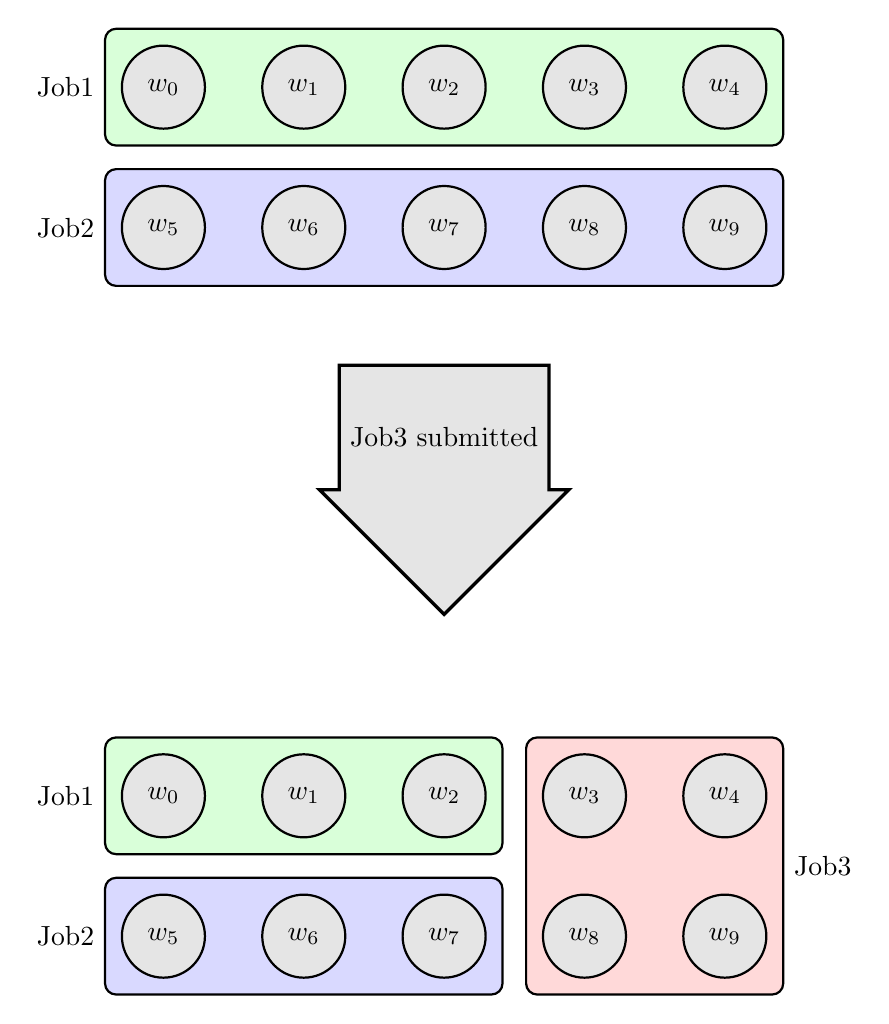
\begin{tikzpicture}
  % Workers on allocation 1
  \matrix (wmtrx1)[worker-matrix]{
	\node(w0){$w_0$};&	\node(w1){$w_1$};&	\node(w2){$w_2$};&	\node(w3){$w_3$};&	\node(w4){$w_4$};\\
	\node(w5){$w_5$};&	\node(w6){$w_6$};&	\node(w7){$w_7$};&	\node(w8){$w_8$};&	\node(w9){$w_9$};\\
  };
  \path (wmtrx1.south) +(0,-2cm) node[single arrow,draw=black,very thick,fill=black!10,minimum height=9em,shape border rotate=270]  {Job3 submitted};

  % Workers on allocation 2

  \matrix [yshift=-9cm](wmtrx2)[worker-matrix]{
	\node(w0_){$w_0$};&	\node(w1_){$w_1$};&	\node(w2_){$w_2$};&	\node(w3_){$w_3$};&	\node(w4_){$w_4$};\\
	\node(w5_){$w_5$};&	\node(w6_){$w_6$};&	\node(w7_){$w_7$};&	\node(w8_){$w_8$};&	\node(w9_){$w_9$};\\
  };

  \begin{pgfonlayer}{background}
    % Allocation 1
	\node [job-1, fit=(w0) (w4)] {};
	\node [job-2, fit=(w5) (w9)] {};

    % Allocation 2
	\node [job-1, fit=(w0_) (w2_)] {};
	\node [job-2, fit=(w5_) (w7_)] {};
	\node [job-3, fit=(w3_) (w9_)] {};
  \end{pgfonlayer}
\end{tikzpicture}

  \caption{Job allocation adjustment}
  \label{fig:allocation-adjustment}
\end{figure}
